\chapter{Son, oscillateurs quantiques et deuxième principe}

\lectureoverview{Le deuxième principe est le point d’arrivée, mais deux calculs concrets nous y préparent. La vitesse du son montre comment des dérivées thermodynamiques deviennent un mouvement observable. L’oscillateur harmonique met ensuite en évidence l’échec de l’équipartition classique pour les degrés de liberté rigides et montre comment la mécanique quantique active les modes un à un. Enfin, nous reviendrons au conflit apparent entre la dynamique microscopique réversible et l’augmentation de l’entropie. Nous nous appuierons sur l’écoulement dans l’espace des phases, le coarse-graining, le chaos et la récurrence pour énoncer le deuxième principe comme une loi extrêmement probable, plutôt que comme une interdiction mécanique sans exception.}

\section{Une promesse au sujet du deuxième principe}

Le problème central est facile à énoncer, mais difficile à expliquer. Les équations newtoniennes sont réversibles : si une évolution microscopique est possible, son évolution renversée dans le temps l’est aussi. Pourtant, le deuxième principe affirme que les processus macroscopiques ont un sens privilégié, caractérisé par une entropie qui, en règle générale, augmente. Nous aborderons cette tension, mais pas tout de suite. Mieux vaut d’abord voir la mécanique statistique fournir des résultats concrets, puis rencontrer, dans le cadre d’un calcul élémentaire, le problème historique qui a contraint la physique classique à céder la place à la physique quantique.

Le premier exemple est numérique et volontairement approximatif : estimons la vitesse du son dans un gaz dilué. Le deuxième est exact dans le cadre de ses hypothèses : calculons l’énergie moyenne d’un oscillateur harmonique dans un bain thermique. L’oscillateur nous conduira de l’équipartition aux niveaux d’énergie quantifiés, d’un mode à une infinité de modes, puis à la question de savoir ce que signifie, pour un système à plusieurs particules, oublier son état initial.

\section{L’échelle moléculaire de la vitesse du son}

Imaginons une légère surdensité dans un gaz dilué. Elle se résorbe parce que des molécules quittent la région où elles sont concentrées ; sa vitesse de propagation devrait donc être comparable à la vitesse moléculaire. L’équipartition donne l’énergie cinétique d’une molécule, \begin{equation}
 \frac{3}{2}k_B T
 =\frac{1}{2}m\expect{v^2},
 \qquad
 \expect{v^2}=\frac{3k_B T}{m}.
 \label{eq:sm7-molecular-speed}
\end{equation}Ici, la température est mesurée à partir du zéro absolu, et \(k_B\) a été rétablie parce que nous voulons utiliser les unités de laboratoire. Il ne s’agit que d’une estimation d’ordre de grandeur : la vitesse quadratique moyenne des molécules n’est pas en soi la vitesse d’une onde sonore collective.

Une dérivation plus systématique considère un petit élément de gaz. Des pressions différentes sur ses faces opposées exercent une force résultante, et son accélération est inversement proportionnelle à la masse volumique. On obtient une expression de la forme \begin{equation}
 c_s^2=
 \left(\frac{\partial P}{\partial \rho_m}\right)_{\cal C},
 \qquad
 \rho_m=m\rho,
 \label{eq:sm7-sound-general}
\end{equation}où \(\rho\) désigne la densité numérique et l’indice \({\cal C}\) précise la condition thermodynamique suivie par la perturbation. Le calcul au tableau utilise \begin{equation}
 P=\rho k_B T
 \quad\Longrightarrow\quad
 \frac{1}{m}
 \left(\frac{\partial P}{\partial\rho}\right)_T
 =\frac{k_B T}{m}.
 \label{eq:sm7-sound-isothermal}
\end{equation}Il s’agit de l’estimation isotherme de la vitesse du son. Elle diffère de \eqref{eq:sm7-molecular-speed} d’un facteur \(3\) pour le carré de la vitesse, ou de \(\sqrt{3}\) pour la vitesse elle-même.

\begin{figure}[t]
\centering
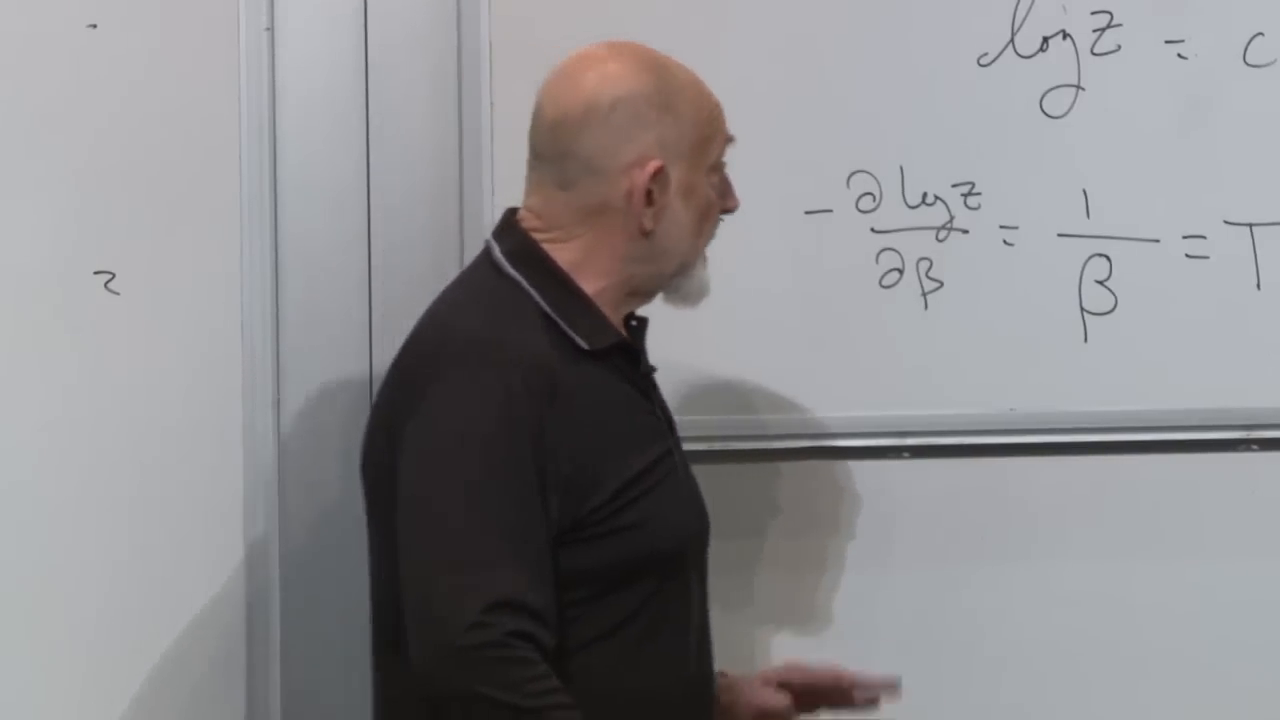
\includegraphics[width=0.90\textwidth]{lecture_07_figure_02.png}
\caption{Estimation de la vitesse moléculaire, dérivée de la pression et substitution du gaz parfait, présentées ensemble.}
\lectureframe{00:08:55}
\end{figure}

Il y a une correction importante à apporter. Une onde sonore de faible amplitude comprime et détend généralement le gaz plus vite que la chaleur ne peut circuler entre les éléments voisins. Le mouvement local est donc approximativement adiabatique, et non isotherme : \begin{equation}
 c_s^2=
 \left(\frac{\partial P}{\partial\rho_m}\right)_S.
 \label{eq:sm7-sound-adiabatic}
\end{equation}Pour un gaz parfait d’indice adiabatique \(\gamma\), \begin{equation}
 P\rho_m^{-\gamma}=\text{constant},
 \qquad
 c_s^2=\gamma\frac{P}{\rho_m}
       =\gamma\frac{k_B T}{m}.
 \label{eq:sm7-sound-ideal-adiabatic}
\end{equation}Pour l’air diatomique à température ambiante, \(\gamma\simeq 7/5\). Le calcul à température fixe constitue donc une première estimation utile, tandis que la dérivée adiabatique apporte la correction physiquement appropriée.

En prenant les valeurs approximatives \begin{equation}
\begin{aligned}
 k_B&\simeq1.3\times10^{-23}\ {\rm J\,K^{-1}},
 &T&\simeq300\ {\rm K},\\
 m_{\rm air}&\simeq4\times10^{-26}\ {\rm kg}.&&
\end{aligned}
 \label{eq:sm7-air-data}
\end{equation}l’estimation moléculaire vaut environ \(500\ {\rm m\,s^{-1}}\). La température doit ici être une température absolue, exprimée en kelvins, et non une échelle décalée comme celle de Fahrenheit. La vitesse du son familière est de l’ordre de \(300\ {\rm m\,s^{-1}}\), et la formule adiabatique du gaz parfait donne environ \(340\ {\rm m\,s^{-1}}\) à température ambiante. Le calcul approximatif a donc permis de trouver le bon ordre de grandeur physique.

\begin{figure}[t]
\centering
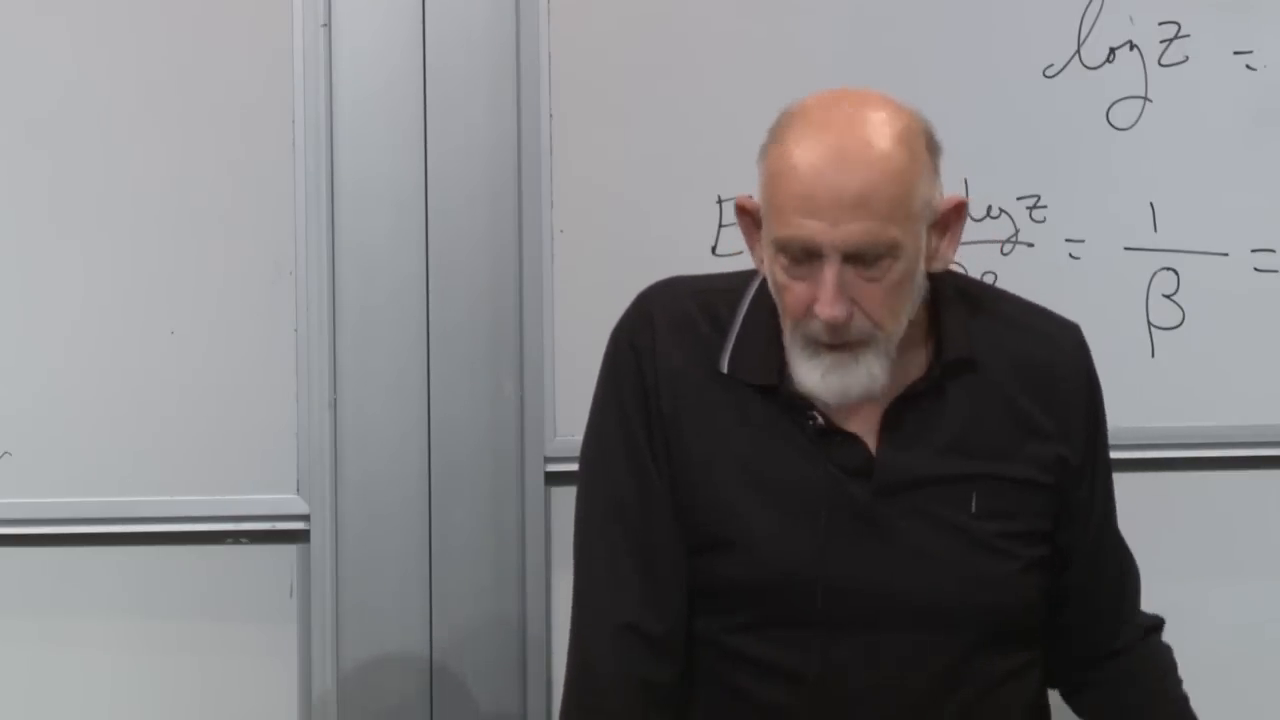
\includegraphics[width=0.90\textwidth]{lecture_07_figure_03.png}
\caption{Estimation pour l’air ambiant à l’aide de la constante de Boltzmann, d’une masse moléculaire effective proche de \(30\) masses du proton et de \(T\simeq300\ {\rm K}\).}
\lectureframe{00:10:55}
\end{figure}

Bien avant qu’une description microscopique soit disponible, on pouvait déterminer la vitesse du son en mesurant la pression en fonction de la densité. Le raisonnement statistique ajoute cette interprétation frappante : la vitesse macroscopique obtenue est fixée par la vitesse thermique des molécules individuelles.

\begin{classroomqa}
\audiencequestion{Faut-il ajouter les neutrons à la masse moléculaire, et le nombre \(14\) pour l’azote compte-t-il seulement les protons ?}
\lecturerresponse{La masse atomique citée compte déjà les protons et les neutrons. Une molécule d’azote contient deux atomes de masse atomique voisine de \(14\) ; sa masse vaut donc environ \(28\) masses du proton. Pour cette estimation, il suffit d’arrondir \(28\) à \(30\).
\lecturetimestamp{00:10:58--00:11:16}}
\end{classroomqa}

\begin{classroomqa}
\audiencequestion{Le facteur \(3\) vient des trois directions de translation, alors que le son se propage dans une seule direction. Faut-il donc supprimer le facteur \(3\) ?}
\lecturerresponse{Cette question nous rappelle à juste titre qu’il ne faut pas confondre la vitesse quadratique moyenne tridimensionnelle des molécules avec une vitesse de propagation unidimensionnelle. L’argument initial ne donnait qu’un ordre de grandeur. Pour obtenir une réponse contrôlée, il faut utiliser la dérivée de la pression et la condition thermodynamique appropriée à l’onde.
\lecturetimestamp{00:11:12--00:12:00}}
\end{classroomqa}

\begin{classroomqa}
\audiencequestion{La dérivée supposait-elle que la température reste constante pendant l’onde ?}
\lecturerresponse{C’était le cas de la substitution affichée pour le gaz parfait. Maintenir la température constante constitue une estimation provisoire plausible pour une perturbation très faible ; la correction usuelle consiste à considérer que le son ordinaire est approximativement adiabatique, ce qui remplace la dérivée isotherme par \(\left(\partial P/\partial\rho_m\right)_S\).
\lecturetimestamp{00:12:59--00:14:01}}
\end{classroomqa}

\begin{classroomqa}
\audiencequestion{Si les variations de pression et de densité sont toutes deux faibles, leur dérivée est-elle alors faible ?}
\lecturerresponse{Non. Une dérivée est le rapport de deux faibles variations dans la limite infinitésimale. \(\delta P\) et \(\delta\rho\) peuvent toutes deux être faibles, tandis que \(\delta P/\delta\rho\) reste finie et fixe la vitesse de l’onde.
\lecturetimestamp{00:14:03--00:14:23}}
\end{classroomqa}

\begin{classroomqa}
\audiencequestion{La vitesse du son devrait-elle augmenter lorsque le gaz est comprimé, comme c’est le cas lorsqu’on passe d’un gaz à un liquide ou à un solide ?}
\lecturerresponse{Oui. La dérivée est évaluée dans l’état considéré, et \(P(\rho,T)\) n’est pas nécessairement une fonction linéaire. Lorsque les molécules sont comprimées et rapprochées, l’équation d’état devient non idéale et \(\partial P/\partial\rho\) peut augmenter considérablement.
\lecturetimestamp{00:14:25--00:15:13}}
\end{classroomqa}

\begin{classroomqa}
\audiencequestion{La valeur \(500\ {\rm m\,s^{-1}}\) est-elle valable à toutes les pressions ?}
\lecturerresponse{Non. Elle correspond au domaine de faible densité, où l’équation du gaz parfait constitue une bonne approximation. Dès que des puissances supérieures de la densité interviennent dans \(P(\rho,T)\), la dérivée, et donc la vitesse du son, dépend de la pression et de la densité.
\lecturetimestamp{00:15:14--00:16:29}}
\end{classroomqa}

\begin{classroomqa}
\audiencequestion{L’image initiale d’un son se propageant à une vitesse approximativement égale à celle des molécules cesse-t-elle aussi d’être valable lorsque la densité augmente ?}
\lecturerresponse{Probablement. Cette image est adaptée à un gaz dilué. Les interactions collectives deviennent de plus en plus importantes à forte densité, ce qui explique précisément pourquoi la dérivée de l’équation d’état constitue la description la plus générale.
\lecturetimestamp{00:16:32--00:16:53}}
\end{classroomqa}

\begin{classroomqa}
\audiencequestion{Pourquoi la masse d’une molécule d’azote a-t-elle été arrondie à environ \(30\) masses du proton plutôt qu’à \(28\) ?}
\lecturerresponse{La précision numérique nécessaire est seulement celle qui convient à l’estimation, donc \(28\) a été arrondi à \(30\). Diviser l’estimation initiale de \(500\ {\rm m\,s^{-1}}\) par \(\sqrt{3}\simeq1.7\) donne également une valeur proche de \(300\ {\rm m\,s^{-1}}\), même si la dérivée adiabatique reste la méthode contrôlée pour calculer la correction.
\lecturetimestamp{00:16:54--00:17:27}}
\end{classroomqa}

\section{Un oscillateur classique dans un bain thermique}

Remplaçons maintenant la molécule en translation libre par un oscillateur harmonique, et considérons tout le reste comme un bain thermique. Une masse attachée à un ressort en est l’image immédiate, mais le modèle est beaucoup plus général. Un mode d’une cavité électromagnétique oscille ; les atomes d’un cristal oscillent ; presque tout système stable légèrement écarté de l’équilibre effectue, au premier ordre, un mouvement harmonique.

Avec \(x\) mesuré depuis la position d’équilibre, la quantité de mouvement \(p\), la masse \(m\) et la constante de raideur \(\kappa\), le hamiltonien s’écrit \begin{equation}
 H(x,p)=\frac{p^2}{2m}+\frac{\kappa x^2}{2},
 \qquad
 \omega=\sqrt{\frac{\kappa}{m}}.
 \label{eq:sm7-classical-hamiltonian}
\end{equation}Le bain fixe \(T\) et, à partir d’ici, nous utilisons de nouveau \(k_B=1\), de sorte que \(\beta=1/T\). Un oscillateur en équilibre avec l’environnement d’une pièce est à une température proche de \(300\ {\rm K}\) ; plongé dans l’hélium liquide, il n’est qu’à quelques kelvins. Un ressort hypothétique placé au centre du Soleil ne resterait pas un ressort, mais l’exemple met en évidence le rôle de l’environnement. Le facteur de Boltzmann se factorise : \begin{equation}
 e^{-\beta H}
 =e^{-\beta p^2/(2m)}
  e^{-\beta\kappa x^2/2}.
 \label{eq:sm7-factorized-weight}
\end{equation}

\begin{figure}[t]
\centering
\includegraphics[width=0.90\textwidth]{lecture_07_figure_04.png}
\caption{Un oscillateur masse-ressort et son hamiltonien, somme des énergies cinétique et potentielle.}
\lectureframe{00:20:55}
\end{figure}

Contrairement au cas du gaz libre, l’intégrale sur la position ne donne pas simplement le volume du récipient. Le potentiel de rappel pondère chaque déplacement : \begin{equation}
 Z_{\rm cl}
 =\frac{1}{h}\int_{-\infty}^{\infty}dp
             \int_{-\infty}^{\infty}dx\,
 e^{-\beta p^2/(2m)}
 e^{-\beta\kappa x^2/2}.
 \label{eq:sm7-classical-z}
\end{equation}Le facteur \(1/h\) rend sans dimension la fonction de partition classique à une dimension. On l’omet dans le calcul au tableau parce qu’il est indépendant de \(\beta\) et ne peut pas influer sur l’énergie moyenne.

\begin{figure}[t]
\centering
\includegraphics[width=0.90\textwidth]{lecture_07_figure_05.png}
\caption{Fonction de partition classique de l’oscillateur, séparée en intégrales gaussiennes sur la quantité de mouvement et le déplacement.}
\lectureframe{00:22:55}
\end{figure}

Pour l’intégrale sur la quantité de mouvement, posons \begin{equation}
 q=\sqrt{\frac{\beta}{2m}}\,p,
 \qquad
 dp=\sqrt{\frac{2m}{\beta}}\,dq.
 \label{eq:sm7-p-gaussian-substitution}
\end{equation}Pour l’intégrale sur la position, posons \begin{equation}
 y=\sqrt{\frac{\beta\kappa}{2}}\,x,
 \qquad
 dx=\sqrt{\frac{2}{\beta\kappa}}\,dy.
 \label{eq:sm7-x-gaussian-substitution}
\end{equation}Comme \(\int_{-\infty}^{\infty}e^{-u^2}\,du=\sqrt{\pi}\), l’intégrale non normalisée sur l’espace des phases utilisée au tableau vaut \begin{equation}
 \int dp\,dx\,e^{-\beta H}
 =\frac{2\pi}{\beta}\sqrt{\frac{m}{\kappa}}
 =\frac{2\pi}{\beta\omega}.
 \label{eq:sm7-classical-z-unnormalized}
\end{equation}En rétablissant la cellule d’espace des phases, on obtient \begin{equation}
 Z_{\rm cl}=\frac{2\pi}{h\beta\omega}
           =\frac{1}{\beta\hbar\omega}.
 \label{eq:sm7-classical-z-normalized}
\end{equation}

Seule la dépendance en \(\beta\) importe pour l’énergie : \begin{equation}
 \begin{aligned}
 \log Z_{\rm cl}&=\text{constant}-\log\beta,\\
 \expect{H}
 &=-\frac{\partial\log Z_{\rm cl}}{\partial\beta}\\
 &=\frac{1}{\beta}=T.
 \end{aligned}
 \label{eq:sm7-classical-energy}
\end{equation}

\begin{figure}[t]
\centering
\includegraphics[width=0.90\textwidth]{lecture_07_figure_06.png}
\caption{L’enchaînement complet du calcul classique au tableau de droite : factorisation gaussienne, \(Z\propto(\beta\omega)^{-1}\) et \(\expect{H}=1/\beta=T\).}
\lectureframe{00:30:15}
\end{figure}

Il n’y a pas de facteur \(3\), car il s’agit d’un oscillateur spatial à une dimension. Il ne reste pas non plus de facteur \(1/2\), car il y a deux termes quadratiques indépendants. Chaque gaussienne contribue \(T/2\) : \begin{equation}
 \expect{K}=\frac{T}{2},
 \qquad
 \expect{U}=\frac{T}{2},
 \qquad
 \expect{H}=T.
 \label{eq:sm7-equipartition-oscillator}
\end{equation}C’est l’équipartition sous sa forme la plus utile : chaque terme quadratique indépendant du hamiltonien classique contribue \(T/2\).

La réponse est indépendante de \(m\) et de \(\kappa\). Le mouvement, lui, dépend de ces paramètres : \begin{equation}
 \expect{p^2}=mT,
 \qquad
 \expect{x^2}=\frac{T}{\kappa},
 \qquad
 \expect{\dot{x}^2}=\frac{T}{m}.
 \label{eq:sm7-classical-fluctuations}
\end{equation}Une masse plus grande se déplace donc plus lentement et un ressort plus rigide a une amplitude plus faible, même si l’énergie moyenne reste égale à \(T\). Cela devient troublant lorsque \(\kappa\) prend une valeur gigantesque. Un ressort trop rigide pour bouger devrait se comporter comme une contrainte figée ; pourtant, l’équipartition classique lui attribue toujours une énergie \(T\).

\begin{classroomqa}
\audiencequestion{Lorsque \(\kappa\to\infty\), la fonction de partition tend vers zéro. Comment peut-on encore utiliser son logarithme ?}
\lecturerresponse{Gardons \(\kappa\) finie, mais arbitrairement grande. Sa contribution à \(\log Z\) est additive et indépendante de \(\beta\), de sorte que la dérivée par rapport à \(\beta\) donne toujours \(T\). Le malaise lié à la limite est réel : le calcul classique est cohérent en lui-même, mais il omet une caractéristique de la nature nécessaire pour décrire les oscillateurs très rigides.
\lecturetimestamp{00:34:01--00:34:54}}
\end{classroomqa}

\begin{classroomqa}
\audiencequestion{La fonction de partition du gaz parfait exigeait un facteur \(N!\). Faut-il un facteur analogue ici ?}
\lecturerresponse{Non. Nous étudions un oscillateur donné, et non la permutation de \(N\) particules identiques. Pour plusieurs modes indépendants étiquetés, les fonctions de partition se multiplient. Le facteur lié à l’indiscernabilité relève d’un autre problème de dénombrement.
\lecturetimestamp{00:35:03--00:35:40}}
\end{classroomqa}

\section{Pourquoi l’équipartition classique a constitué une crise}

Les molécules réelles ne sont pas des points sans structure. Une molécule diatomique possède une liaison susceptible de vibrer, donc un oscillateur interne. Un dénombrement classique naïf attribuerait à ce mode une énergie thermique supplémentaire, même aux températures ordinaires. Dans un dénombrement volontairement schématique, l’activation d’un oscillateur vibrationnel fait passer une énergie de \(3T/2\) à environ \(5T/2\). Pour établir précisément le bilan de chaleur, il faut aussi tenir compte des degrés de liberté de rotation et distinguer l’énergie de sa dérivée par rapport à la température. Le fait expérimental décisif est plus simple : à basse température, les modes internes rigides ne contribuaient pas, contrairement à ce qu’exigeait l’équipartition classique.

On pourrait nier que la molécule possède une structure interne, ce qui serait absurde, ou reconnaître qu’il manque un ingrédient à la mécanique classique. Cet ingrédient, c’est la mécanique quantique. Nous n’en avons besoin que d’un aspect : les niveaux d’énergie d’un oscillateur harmonique sont régulièrement espacés.

\section{L’oscillateur quantique}

Commençons par décaler l’origine des énergies et écrivons le spectre d’excitation sous la forme \begin{equation}
 E_n^{\rm exc}=n\hbar\omega,
 \qquad n=0,1,2,\ldots.
 \label{eq:sm7-shifted-spectrum}
\end{equation}La fonction de partition est désormais une véritable somme, et non plus une intégrale sur l’espace des phases : \begin{align}
 Z_{\rm exc}
 &=\sum_{n=0}^{\infty}e^{-\beta n\hbar\omega} \notag\\
 &=1+x+x^2+\cdots
  =\frac{1}{1-x},
 \qquad x=e^{-\beta\hbar\omega}, \notag\\
 &=\frac{1}{1-e^{-\beta\hbar\omega}}.
 \label{eq:sm7-quantum-z}
\end{align}

\begin{figure}[t]
\centering
\includegraphics[width=0.90\textwidth]{lecture_07_figure_07.png}
\caption{Niveaux régulièrement espacés et calcul de la fonction de partition de l’oscillateur quantique à l’aide d’une série géométrique.}
\lectureframe{00:42:05}
\end{figure}

La dérivation donne l’énergie moyenne d’excitation : \begin{align}
 E_{\rm exc}
 &=-\frac{\partial\log Z_{\rm exc}}{\partial\beta}
  =-\frac{1}{Z_{\rm exc}}
    \frac{\partial Z_{\rm exc}}{\partial\beta}
 \notag\\
 &=\hbar\omega\,
   \frac{e^{-\beta\hbar\omega}}
        {1-e^{-\beta\hbar\omega}}
  =\frac{\hbar\omega}{e^{\beta\hbar\omega}-1}.
 \label{eq:sm7-quantum-energy}
\end{align}

\begin{figure}[t]
\centering
\includegraphics[width=0.90\textwidth]{lecture_07_figure_08.png}
\caption{Énergie thermique d’excitation obtenue par dérivation de la fonction de partition quantique par rapport à \(\beta\).}
\lectureframe{00:46:05}
\end{figure}

\subsection{Haute température}

Lorsque \(\beta\hbar\omega\ll1\), \begin{equation}
 e^{-\beta\hbar\omega}
 =1-\beta\hbar\omega
  +O\!\left((\beta\hbar\omega)^2\right).
 \label{eq:sm7-high-t-expansion}
\end{equation}Le numérateur de \eqref{eq:sm7-quantum-energy} tend vers \(\hbar\omega\), tandis que le dénominateur vaut, au premier ordre, \(\beta\hbar\omega\). Par conséquent, \begin{equation}
 E_{\rm exc}\simeq\frac{1}{\beta}=T.
 \label{eq:sm7-high-t-energy}
\end{equation}La réponse quantique retrouve l’équipartition classique lorsque l’énergie thermique couvre de nombreux intervalles entre niveaux.

\subsection{Basse température}

Lorsque \(\beta\hbar\omega\gg1\), l’exponentielle est très petite : \begin{equation}
 E_{\rm exc}
 \simeq\hbar\omega e^{-\beta\hbar\omega}.
 \label{eq:sm7-low-t-energy}
\end{equation}L’excitation thermique de l’oscillateur est supprimée de façon exponentielle. Dans la convention où l’origine de l’énergie est décalée, elle est presque nulle ; nous rétablirons plus bas l’énergie de point zéro physique.

\begin{figure}[t]
\centering
\includegraphics[width=0.90\textwidth]{lecture_07_figure_09.png}
\caption{Développement à basse température : la première excitation thermique est supprimée par le facteur \(e^{-\beta\hbar\omega}\).}
\lectureframe{00:51:55}
\end{figure}

Le passage d’un régime à l’autre se produit lorsque \begin{equation}
 \beta\hbar\omega\sim1,
 \qquad\text{or equivalently}\qquad
 T\sim\hbar\omega.
 \label{eq:sm7-crossover}
\end{equation}Cette condition a une signification directe. L’équipartition classique attribuerait à l’oscillateur une énergie \(T\). Les effets quantiques deviennent incontournables lorsque cette échelle passe sous l’intervalle entre deux niveaux. On a donc \begin{equation}
\begin{aligned}
 \hbar\omega\gg T&:\quad \text{frozen and quantum},\\
 \hbar\omega\ll T&:\quad \text{active and classical}.
\end{aligned}
 \label{eq:sm7-regimes}
\end{equation}Un ressort plus rigide a une valeur de \(\omega=\sqrt{\kappa/m}\) plus grande ; il faut donc une température plus élevée pour que son comportement devienne classique.

\section{Les degrés de liberté apparaissent quand on chauffe la matière}

À basse température, une molécule diatomique peut se comporter thermiquement comme une particule ponctuelle, car la vibration de sa liaison rigide est gelée. Lorsque \(T\) augmente et franchit \(\hbar\omega\), le mode vibrationnel s’active. Les modes de rotation peuvent s’activer à une échelle plus basse ; à des températures encore plus élevées, d’autres mouvements internes deviennent accessibles et l’atome finit par s’ioniser. Chauffer ne revient pas simplement à ajouter de l’énergie à une liste fixe de modes. Cela révèle des degrés de liberté qui étaient invisibles à plus basse température.

Une molécule imaginaire à structure emboîtée précise cette idée. Deux atomes sont reliés par un ressort rigide, et l’un de ces atomes apparents est lui-même une paire reliée par un ressort encore plus rigide. À basse température \(T\), les deux structures semblent ponctuelles. Au premier seuil, la vibration externe apparaît ; au second, la structure interne devient visible. La complexité du système se dévoile à mesure que l’énergie franchit chaque échelle.

\begin{classroomqa}
\audiencequestion{Une fois que l’oscillateur est déjà dans le régime classique, le fait de chauffer davantage tend-il le ressort ou modifie-t-il sa fréquence ?}
\lecturerresponse{Non. La constante de raideur et la fréquence restent fixes. Une température plus élevée accroît les quantités de mouvement et les amplitudes typiques, et donc l’énergie. La rigidité détermine la température à laquelle la loi classique commence à s’appliquer ; elle ne signifie pas que le ressort se tend davantage avec la température.
\lecturetimestamp{01:03:17--01:05:11}}
\end{classroomqa}

\subsection{Cristaux et chaleur spécifique d’Einstein}

Un cristal contient un grand nombre de modes vibrationnels. L’équipartition classique attribue une énergie de l’ordre de \(T\) à chaque oscillateur actif et surestime donc la chaleur spécifique à basse température. Le modèle d’Einstein de 1907 traitait les vibrations du cristal par la mécanique quantique et expliquait pourquoi elles sont supprimées jusqu’à ce que l’énergie thermique atteigne l’intervalle entre les niveaux. Les modèles de physique du solide plus précis prennent en compte une distribution de fréquences des modes, mais le principe du gel des modes apparaît déjà dans le calcul d’Einstein.

\begin{classroomqa}
\audiencequestion{Einstein a-t-il reçu le prix Nobel pour ces travaux, et ceux-ci ne datent-ils que d’après l’établissement de la mécanique quantique ?}
\lecturerresponse{Non. La citation du prix Nobel portait sur l’effet photoélectrique. Le modèle de chaleur spécifique a été publié en 1907, bien avant que les fondements complets de la mécanique quantique soient compris. Einstein a accepté et développé des idées quantiques cruciales, même s’il a ensuite contesté certains aspects de la théorie parvenue à maturité.
\lecturetimestamp{00:58:38--01:03:16}}
\end{classroomqa}

\begin{classroomqa}
\audiencequestion{La mécanique statistique classique remplace une somme sur des états discrets par une intégrale apparemment uniforme sur les positions et les quantités de mouvement. Comment justifier ce dénombrement des états ?}
\lecturerresponse{La justification ultime vient de la mécanique quantique. À haute température, \[
 Z_{\rm exc}\simeq\frac{1}{\beta\hbar\omega},
\]ce qui correspond exactement au résultat classique sans dimension \eqref{eq:sm7-classical-z-normalized}. Lorsque l’intervalle entre niveaux n’est pas résolu, les cellules quantiques de l’espace des phases donnent la mesure classique de cet espace.
\lecturetimestamp{00:59:38--01:03:06}}
\end{classroomqa}

\subsection{Une corde contient une infinité d’oscillateurs}

Une corde de violon ou de guitare se décompose en modes normaux : le fondamental, les harmoniques supérieures et des longueurs d’onde de plus en plus courtes. Mathématiquement, elle comporte une infinité de modes oscillatoires. Si l’équipartition classique attribuait une énergie \(T\) à chacun d’eux, l’énergie de la corde à l’équilibre thermique serait infinie. La mécanique quantique évite cette catastrophe. Les modes de longueur d’onde la plus courte ont les fréquences les plus élevées et restent gelés à toute température finie ; un nombre croissant de modes s’active à mesure que \(T\) augmente. Le même raisonnement sera plus tard à la base du rayonnement du corps noir.

\begin{figure}[t]
\centering
\includegraphics[width=0.90\textwidth]{lecture_07_figure_10.png}
\caption{Superposition de plusieurs modes normaux sur une corde, illustrant pourquoi une corde continue constitue un ensemble infini d’oscillateurs harmoniques.}
\lectureframe{01:09:30}
\end{figure}

\begin{classroomqa}
\audiencequestion{Peut-on observer directement le passage du régime quantique au régime classique, et le chauffage peut-il inverser le comportement à basse température ?}
\lecturerresponse{Oui. La dépendance en température de la chaleur spécifique d’un cristal rend directement mesurables le gel des modes vibrationnels, puis leur activation.
\lecturetimestamp{01:09:11--01:10:13}}
\end{classroomqa}

\begin{classroomqa}
\audiencequestion{Pour un grand nombre d’oscillateurs, répète-t-on la fonction de partition d’un oscillateur pour chaque mode ?}
\lecturerresponse{Pour des modes indépendants, \[
\begin{aligned}
 Z_{\rm tot}&=\prod_j Z_j,&
 \log Z_{\rm tot}&=\sum_j\log Z_j,\\
 E_{\rm tot}&=\sum_j E_j.&&
\end{aligned}
\]Les modes tels que \(\hbar\omega_j\gg T\) apportent une contribution thermique exponentiellement faible ; ceux dont la fréquence se situe sous le seuil contribuent de façon appréciable.
\lecturetimestamp{01:10:14--01:11:00}}
\end{classroomqa}

\begin{classroomqa}
\audiencequestion{Qu’est-il advenu de l’énergie de point zéro \(\hbar\omega/2\) de l’oscillateur ?}
\lecturerresponse{Les niveaux physiques sont \[
 E_n=\left(n+\frac12\right)\hbar\omega.
\]Par conséquent, \[
 \begin{aligned}
 Z_{\rm phys}
 &=e^{-\beta\hbar\omega/2}Z_{\rm exc},\\
 E_{\rm phys}
 &=\frac{\hbar\omega}{2}
  +\frac{\hbar\omega}{e^{\beta\hbar\omega}-1}.
 \end{aligned}
\]Ce décalage commun ne modifie ni les probabilités des niveaux, ni l’entropie, ni la capacité thermique, ni l’énergie d’excitation thermique, mais il décale l’énergie moyenne absolue de \(\hbar\omega/2\). Le facteur multiplicatif dans \(Z\) dépend de \(\beta\) ; il ne faut donc pas le supprimer lorsqu’on cherche l’énergie absolue.
\lecturetimestamp{01:11:08--01:11:37}}
\end{classroomqa}

\section{Le deuxième principe, énigme de la réversibilité}

Nous pouvons maintenant revenir au problème annoncé. Le deuxième principe affirme que l’évolution macroscopique ordinaire est irréversible et que l’entropie tend à augmenter. L’évolution hamiltonienne microscopique est réversible. Comment une application réversible sur les états exacts peut-elle produire une loi irréversible pour les états macroscopiques ?

Représentons le système par un point dans un espace des phases de grande dimension, \[
 \Gamma=(q_1,\ldots,q_N,p_1,\ldots,p_N).
\]Notre connaissance ne porte généralement pas sur un point exact. Supposons qu’elle soit décrite par une densité de probabilité uniforme sur un domaine compact \(A\) de volume \(\Omega_A\) : \begin{equation}
 f(\Gamma)=
 \begin{cases}
  1/\Omega_A,&\Gamma\in A,\\
  0,&\Gamma\notin A.
 \end{cases}
 \label{eq:sm7-uniform-blob}
\end{equation}Dans les unités où \(k_B=1\), son entropie de Gibbs à grain fin vaut \begin{equation}
 S_{\rm fine}
 =-\int d\Gamma\,f\log f
 =\log\Omega_A.
 \label{eq:sm7-blob-entropy}
\end{equation}Un domaine plus petit signifie davantage d’information et une entropie plus faible. Le signe est ainsi fixé : une incertitude croissante élargit la région occupée et augmente \(\log\Omega_A\).

\begin{figure}[t]
\centering
\includegraphics[width=0.90\textwidth]{lecture_07_figure_11.png}
\caption{Domaine compact de probabilité dans une coupe schématique bidimensionnelle de l’espace des phases complet des positions et des quantités de mouvement.}
\lectureframe{01:20:20}
\end{figure}

\begin{classroomqa}
\audiencequestion{Le système est-il physiquement contraint de rester dans le domaine dessiné, et est-il déjà à l’équilibre ?}
\lecturerresponse{Non. Le domaine décrit ce que l’on sait de l’état initial ; ce n’est pas une paroi dans l’espace des phases. Il n’est pas nécessairement une distribution d’équilibre. Un gaz initialement confiné dans un réservoir situé dans un coin d’une pièce est un exemple concret d’information particulière, hors équilibre.
\lecturetimestamp{01:14:55--01:15:24}}
\end{classroomqa}

\section{Écoulement de Liouville et augmentation après coarse-graining}

Le théorème de Liouville affirme que l’écoulement hamiltonien préserve le volume dans l’espace des phases. Le domaine exact peut se déplacer, s’étirer, se replier et devenir extrêmement mince, mais \begin{equation}
 \Omega_{A(t)}=\Omega_{A(0)},
 \qquad
 S_{\rm fine}(t)=S_{\rm fine}(0).
 \label{eq:sm7-liouville}
\end{equation}L’analogue discret est une permutation réversible des états. Si l’on sait initialement qu’un dé se trouve dans l’un de deux états, une évolution bijective peut changer lesquels sont possibles, mais elle ne modifie pas leur nombre.

Les descriptions réelles ont une résolution finie. La mécanique quantique fournit une cellule naturelle dans l’espace des phases, tandis qu’une expérience classique a une capacité de mesure finie, même sans faire appel à la théorie quantique. Sous l’effet de l’écoulement hamiltonien, le domaine peut devenir un long filament mince et sinueux. Si l’écart entre deux replis voisins passe sous le seuil de résolution, nous remplaçons chaque voisinage non résolu par une cellule grossière. Le volume exact occupé reste constant, mais l’union des cellules grossières s’agrandit : \begin{equation}
 \Omega_{\rm coarse}(t)\geq\Omega_{A(t)},
 \qquad
 S_{\rm coarse}(t)=\log\Omega_{\rm coarse}(t).
 \label{eq:sm7-coarse-entropy}
\end{equation}

\begin{figure}[t]
\centering
\includegraphics[width=0.90\textwidth]{lecture_07_figure_12.png}
\caption{Un filament qui préserve le volume, observé à travers des cellules de résolution finie. Le filament noir exact conserve son aire ; les cellules grossières rouges couvrent une région effective plus grande.}
\lectureframe{01:22:10}
\end{figure}

\begin{classroomqa}
\audiencequestion{Les cellules grossières se chevauchent. Cela contredit-il le théorème de Liouville ?}
\lecturerresponse{Non. Le théorème de Liouville s’applique au filament exact, qui reste bijectif et préserve le volume. Le chevauchement est propre à notre description floutée : nous avons écarté l’information qui permettrait de savoir sur quel filament mince se trouve l’état.
\lecturetimestamp{01:21:32--01:21:50}}
\end{classroomqa}

Une analogie utile est celle du coton. Le volume matériel de toutes ses fibres peut rester presque constant tandis qu’un amas de fibres étirées occupe un grand volume apparent aux yeux d’un observateur incapable de distinguer chaque fibre. De même, un domaine de l’espace des phases développe des tentacules de plus en plus fins, qui en développent à leur tour d’autres encore plus fins. Toute résolution finie fixe finit par ne plus permettre de les suivre.

\begin{classroomqa}
\audiencequestion{L’entropie semble-t-elle simplement augmenter en mécanique classique, tandis que la mécanique quantique rend cette augmentation réelle en imposant une limite fondamentale de résolution ?}
\lecturerresponse{L’argument du coarse-graining n’exige aucune limite quantique. L’entropie dépend à la fois du système et des distinctions macroscopiques conservées dans sa description. Si l’on dispose d’une information microscopique infinie, l’entropie à grain fin reste constante ; à toute résolution finie fixe, les filaments chaotiques finissent par devenir indiscernables, et l’entropie après coarse-graining augmente.
\lecturetimestamp{01:24:04--01:25:20}}
\end{classroomqa}

\section{Chaos, région accessible finie et mise à l’équilibre}

Dans une boîte, les positions d’un gaz sont bornées. À énergie totale finie fixée, les quantités de mouvement le sont également, même si toute l’énergie se concentre momentanément sur une seule particule. Sous les hypothèses habituelles de confinement, la coquille d’énergie accessible dynamiquement a donc une mesure finie.

\begin{figure}[t]
\centering
\includegraphics[width=0.90\textwidth]{lecture_07_figure_13.png}
\caption{Région bornée de l’espace des phases accessible, à côté du filament et de sa représentation après coarse-graining.}
\lectureframe{01:28:10}
\end{figure}

Dans un système chaotique, des points initiaux proches suivent des évolutions semblables pendant un certain temps, puis s’écartent. Lors d’une casse au billard, une variation imperceptible de la direction de la bille blanche se répercute sur les collisions suivantes ; les écarts s’amplifient jusqu’à ce que les configurations finales n’aient plus rien en commun. Une région initiale entière est donc étirée et repliée dans la région accessible. À résolution finie, elle tend vers une description d’équilibre étendue et presque uniforme.

\begin{figure}[t]
\centering
\includegraphics[width=0.90\textwidth]{lecture_07_figure_14.png}
\caption{Un état initial particulier, compact, évolue en un filament complexe dans la région accessible bornée, tandis que les cellules de la description à gros grains s’étalent sur une aire beaucoup plus grande.}
\lectureframe{01:33:10}
\end{figure}

Deux réserves s’imposent. Le chaos, à lui seul, ne prouve pas que chaque trajectoire visite tout voisinage accessible ; cette affirmation plus forte concernant l’exploration de l’espace requiert une propriété d’ergodicité ou de mélange. Par ailleurs, les systèmes physiques ne sont pas tous chaotiques. Un gaz générique à plusieurs corps et des billards idéalisés constituent le cadre visé, où le mélange est une attente physique raisonnable.

\section{La récurrence n’abolit pas l’irréversibilité}

Supposons que toutes les molécules d’air se trouvent initialement dans un coin, avec une distribution des vitesses préparée spécialement. Les collisions les dispersent rapidement dans la pièce, et la description à gros grains atteint l’équilibre. Dans un espace des phases fini qui préserve la mesure, le théorème de récurrence de Poincaré affirme que presque tout point initial revient arbitrairement près de son point de départ. Pour une tolérance \(\epsilon>0\), un temps de récurrence \(t_R(\epsilon)\) est fini sous les hypothèses du théorème, bien qu’il soit fabuleusement long pour un système macroscopique. Un retour exact à un point défini avec une précision infinie n’est ni nécessaire ni généralement attendu.

\begin{classroomqa}
\audiencequestion{Dans l’exemple du billard, le fait de frapper la bille blanche lui apporte-t-il de l’énergie et compromet-il l’évolution d’un système isolé ?}
\lecturerresponse{L’état initial choisi correspond à l’instant qui suit immédiatement le coup, cette énergie étant déjà prise en compte. La récurrence concerne l’évolution ultérieure du billard idéalisé et isolé ; un retour près de l’état initial comprend une configuration équivalente à celle où la bille blanche s’approche du triangle de billes dans la limite de la tolérance choisie.
\lecturetimestamp{01:35:37--01:35:55}}
\end{classroomqa}

\begin{classroomqa}
\audiencequestion{Si le gaz peut finir par revenir dans le coin, avons-nous perdu de l’information, et le système est-il vraiment réversible ?}
\lecturerresponse{La dynamique microscopique reste réversible en permanence. L’entropie à gros grains peut augmenter parce que nous cessons de résoudre les corrélations fines, mais une fluctuation exceptionnellement rare peut ramener le système près de son état macroscopique initial particulier. Récurrence et irréversibilité à gros grains sont donc compatibles.
\lecturetimestamp{01:37:34--01:38:15}}
\end{classroomqa}

Cela conduit à la formulation essentielle de Boltzmann. L’entropie n’augmente pas à chaque instant logiquement possible. Pour un état macroscopique de non-équilibre d’un grand système, les évolutions microscopiques compatibles qui conduisent vers des états macroscopiques d’entropie plus élevée sont de très loin les plus nombreuses, comparées à celles qui mènent vers des états encore plus particuliers. L’entropie \emph{augmente probablement}. Les fluctuations vers le bas et les récurrences sont possibles, mais leurs probabilités et leurs échelles de temps les rendent imperceptibles dans l’expérience macroscopique ordinaire. Le problème de la réversibilité fut l’un des grands débats historiques de la mécanique statistique et pesa lourdement sur Boltzmann. Ce lien historique ne doit pas être transformé en une simple affirmation causale sur sa vie.

\section{Ce que signifie le chaos}

Pour donner une définition plus opérationnelle du chaos, supposons que deux points initiaux de l’espace des phases diffèrent de \(\delta\Gamma(0)\) ; dans une direction chaotique, on a typiquement
\begin{equation}
 \lVert\delta\Gamma(t)\rVert
 \sim e^{\lambda t}\lVert\delta\Gamma(0)\rVert,
 \qquad \lambda>0,
 \label{eq:sm7-lyapunov-growth}
\end{equation}
dans le régime où la séparation linéarisée a un sens. Le nombre \(\lambda\) est un exposant de Lyapunov. Pour prévoir l’évolution jusqu’à un temps \(t\), la précision requise sur les données initiales est approximativement proportionnelle à \(e^{-\lambda t}\). La précision des lois dynamiques compte également : les erreurs du modèle sont amplifiées au même titre que celles des conditions initiales. La météo en est l’exemple familier.

\begin{classroomqa}
\audiencequestion{Existe-t-il un principe selon lequel \emph{la plupart des} systèmes sont chaotiques, ou est-ce simplement empirique ?}
\lecturerresponse{Il existe une infinité de Hamiltoniens chaotiques et non chaotiques, et même le mot \emph{plupart} suppose une mesure sur l’espace des Hamiltoniens. Les systèmes complexes en interaction sont souvent chaotiques, mais il n’existe pas de critère universel élémentaire permettant de classer chaque Hamiltonien par simple inspection.
\lecturetimestamp{01:39:27--01:40:49}}
\end{classroomqa}

\begin{classroomqa}
\audiencequestion{Que signifie précisément \emph{chaotique} dans cette discussion ?}
\lecturerresponse{Les trajectoires de phase proches s’écartent assez rapidement pour que la prévision à long terme exige une connaissance des conditions initiales dont la précision s’améliore de façon exponentielle. L’oscillateur harmonique offre un contraste : les points de phase voisins tournent ensemble et restent proches. Le problème exact de Kepler à deux corps est lui aussi non chaotique, tandis que le problème général à trois corps comporte des régimes chaotiques.
\lecturetimestamp{01:40:50--01:43:45}}
\end{classroomqa}

\begin{classroomqa}
\audiencequestion{Faut-il connaître avec une grande précision les lois du mouvement ainsi que les conditions initiales ?}
\lecturerresponse{Oui. Les deux sources d’erreur se propagent dans la dynamique, et l’évolution chaotique les amplifie toutes les deux.
\lecturetimestamp{01:43:46--01:43:55}}
\end{classroomqa}

Le pendule double en fournit un exemple saisissant. Un pendule ordinaire est intégrable et prévisible. Ajoutons un second pendule : des trajectoires qui commencent presque au même endroit peuvent finir par transférer l’énergie différemment et prendre des directions tout à fait distinctes.

\begin{figure}[t]
\centering
\includegraphics[width=0.90\textwidth]{lecture_07_figure_15.png}
\caption{Le pendule double, exemple concret de chaos déterministe.}
\lectureframe{01:44:40}
\end{figure}

\begin{classroomqa}
\audiencequestion{Pourquoi un système mécanique peut-il être chaotique alors qu’un autre ne l’est pas ?}
\lecturerresponse{C’est une propriété du Hamiltonien et de ses structures invariantes, et non une conséquence du frottement ou du bruit expérimental. La déterminer peut être mathématiquement difficile ; la complexité est un indice, mais pas une preuve.
\lecturetimestamp{01:44:03--01:45:58}}
\end{classroomqa}

\begin{classroomqa}
\audiencequestion{Un pendule double idéal reste-t-il chaotique en l’absence de frottement ?}
\lecturerresponse{Oui. La dissipation n’est pas nécessaire. Un mouvement hamiltonien exact et déterministe peut présenter une dépendance sensible aux conditions initiales. Des conditions initiales connues avec une précision infinie détermineraient la trajectoire indéfiniment, mais une précision finie limite la durée de prévision.
\lecturetimestamp{01:45:57--01:47:54}}
\end{classroomqa}

\begin{classroomqa}
\audiencequestion{Le chaos revient-il à ne pas avoir de solution sous forme fermée ?}
\lecturerresponse{Non. En général, les systèmes chaotiques ne possèdent pas de trajectoire globale utile sous forme fermée, mais la résolubilité analytique et la dépendance sensible sont des propriétés distinctes. Le chaos se diagnostique par la séparation des trajectoires, et non par notre seule incapacité à écrire une formule.
\lecturetimestamp{01:48:20--01:49:23}}
\end{classroomqa}

\begin{classroomqa}
\audiencequestion{En quoi le chaos omniprésent diffère-t-il du fait de tenir exactement en équilibre au sommet instable d’une colline ?}
\lecturerresponse{Le sommet de la colline correspond à un unique état instable exceptionnel : lorsqu’on s’en éloigne, les trajectoires proches ne sont pas nécessairement amenées à diverger rapidement. Dans une région chaotique, l’instabilité est typique le long de l’orbite et les points de phase voisins s’écartent à plusieurs reprises. Un exposant de Lyapunov positif caractérise cette croissance persistante.
\lecturetimestamp{01:49:27--01:50:11}}
\end{classroomqa}

\section{Du mouvement microscopique aux lois statistiques}

L’estimation de la vitesse du son a montré comment le mouvement thermique microscopique fixe une échelle macroscopique de propagation, tandis que les questions ont mis en évidence la dérivée thermodynamique qu’il faut spécifier. L’oscillateur a ensuite illustré à la fois la portée et les limites de l’équipartition classique. L’espacement des niveaux quantiques gèle les modes raides, explique pourquoi les capacités calorifiques varient avec la température et empêche qu’une infinité de modes de haute fréquence porte une énergie thermique infinie.

Cette même progression, de la microphysique exacte à la description macroscopique effective, résout la contradiction apparente au cœur du second principe. L’écoulement hamiltonien préserve exactement le volume de l’espace des phases et reste réversible. L’étirement chaotique engendre des corrélations plus fines que ne peut conserver une description macroscopique, de sorte que la région occupée à gros grains s’agrandit. La récurrence garantit que les retours rares ne sont pas interdits ; la probabilité explique pourquoi ils ne caractérisent pas l’expérience ordinaire. Le second principe n’est pas une nouvelle force microscopique irréversible. Il exprime la direction statistique d’évolution, d’une fiabilité écrasante, pour des conditions initiales macroscopiques particulières dans des systèmes comportant un nombre immense de degrés de liberté.